\documentclass{article}
\usepackage{tikz}
\usetikzlibrary{arrows,decorations.pathmorphing,backgrounds,positioning,fit,petri}
\begin{document}
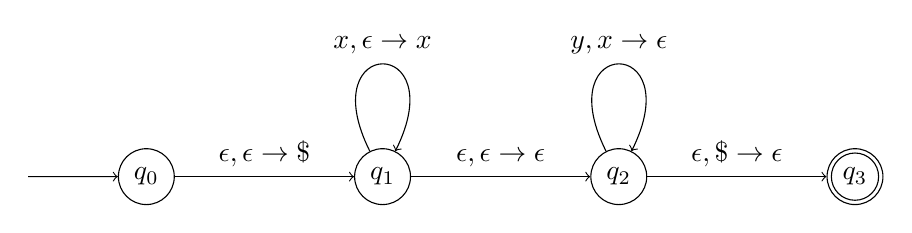
\begin{tikzpicture}[scale=3,
   state/.style={circle, radius=0.14},
   final/.style={radius=0.1}]
   \node (q0) at (1,1) [draw, state] {$q_0$};
   \node (q1) at (2,1) [draw, state] {$q_1$};
   \node (q2) at (3,1) [draw, state] {$q_2$};
   \node (q3) at (4,1) [draw, state, final] {$q_3$};
   \draw (q3) circle[final];
   \draw (0.5,1)[->] -- (q0);
   \draw (q0)[->] -- node[above]{$\epsilon,\epsilon\to \$$} (q1);
   \draw (q1)[->] -- node[above]{$\epsilon,\epsilon\to \epsilon$} (q2);
   \draw (q2)[->] -- node[above]{$\epsilon,\$\to \epsilon$} (q3);
   \draw (q1)[->] .. controls +(-0.3,0.6) and +(0.3,0.6) .. node[above]{$x,\epsilon\to x$} (q1);
   \draw (q2)[->]  .. controls +(-0.3,0.6) and +(0.3,0.6) .. node[above]{$y,x\to \epsilon$} (q2);
\end{tikzpicture}
\end{document}
